\section{Introduction}
%(2 pages)}
\label{sec:intro}

\leanparagraph{Motivation}
Recent advances in information extraction have led to
huge graph-structured knowledge bases (KBs) also known as knowledge graphs (KGs) such as NELL \cite{nell}, DBpedia \cite{dbpedia}, YAGO \cite{yago} and Wikidata \cite{wikidata}. These KGs contain millions or billions of relational facts in the form of subject-predicate-object (SPO) triples, e.g., $\tuple{\mi{clara\;isMarriedTo\;dave}}$ or $\tuple{\mi{dave\;isA\;researcher}}$. Such triples can be straightforwardly represented by mesna of positive unary and binary first-order logic facts, e.g. $\mi{marriedTo(clara,dave)}$ and $\mi{researcher(dave)}$.

An important task over KGs is rule learning, which is relevant for a variety of applications ranging from knowledge graph curation (completion, error detection) \cite{DBLP:journals/semweb/Paulheim17} to data mining and semantic culturonomics. Rules over KGs are of the form $\mi{head \leftarrow body}$, where $\mi{head}$ is a binary atom and $\mi{body}$ is a conjunction of, possibly negated, binary and unary atoms. 
Traditionally, rule induction has been studied in the context of relational data mining (see e.g., \cite{amie,op,rdf2rules}). The methods from this area can be used to identify prominent patterns from KGs, such as \emph{``Married people live in the same
place''}, and cast them in the form of Horn rules, such as:
$\mi{r_1:\;}\mi{livesIn(Y,Z)}\leftarrow \mi{isMarriedTo(X,Y),livesIn(X,Z)}$.

For the KG curation, this has two-fold benefits. First, since KGs operate under the Open World
Assumption (OWA) (i.e., absent facts are treated as unknown rather than false),
the rules can be used to derive additional facts. For example, applying the rule
$\mi{r_1}$ mined from the graph in Figure~\ref{rdf}, the missing living places of Dave and Lucy can be deduced based on the data about their spouses. Second, rules can be used to eliminate erroneous facts in the KG. For example, assuming that $\mi{livesIn}$ is a functional relation, Amsterdam as a living place of
Alice could be questioned as it differs from her husband's.

\begin{figure}[t]
\centering
\begin{subfigure}[b]{0.75\textwidth}
    \centering
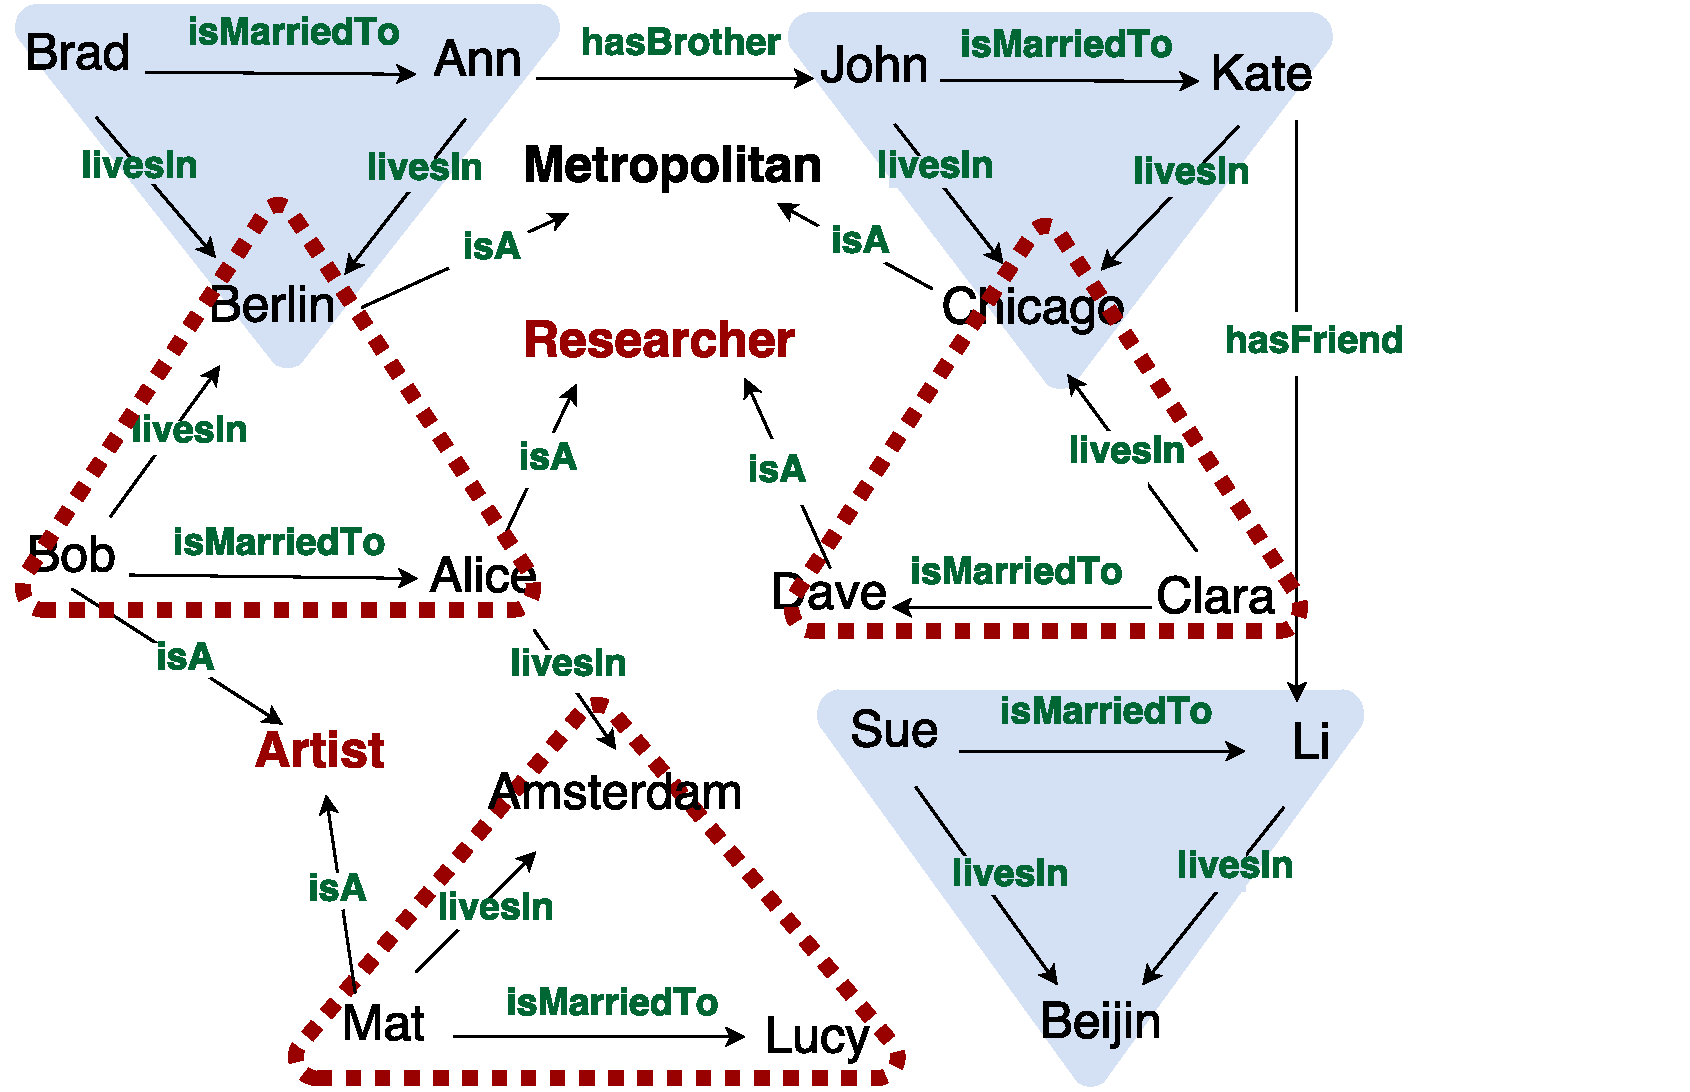
\includegraphics[width=0.7\textwidth]{figures/kg_extended}
\caption{Rule mining for KG completion and KG cleaning}
\label{rdf}
\end{subfigure}
\begin{subfigure}[b]{0.24\textwidth}
\scriptsize
\renewcommand*{\arraystretch}{0.95}
\begin{tabular}{|l|l|l|l|l|l|l|l|l|}
\hline
&  \rot{$\mi{bornInUS}$} &\rot{$\mi{livesInUS}$}&
\rot{$\mi{stateless}$}&\rot{$\mi{immigrant}$}&\rot{$\mi{singer}$}&\rot{$\mi{poet}$}&\rot{$\mi{hasUSPass}$}\\ \hline
$\mi{p1}$ & $\checkmark$ &$\checkmark$ &&&$\checkmark$&&$\checkmark$ \\ \hline
$\mi{p2}$ & $\checkmark$ &$\checkmark$ &&&&&$\checkmark$ \\ \hline
$\mi{p3}$ & $\checkmark$ &$\checkmark$ &&&$\checkmark$&$\checkmark$&$\checkmark$ \\ \hline
$\mi{p4}$ & $\checkmark$ &$\checkmark$ &&&&&$\checkmark$ \\ \hline
$\mi{p5}$ & $\checkmark$ &$\checkmark$ &$\checkmark$&&&& \\ \hline
$\mi{p6}$ & $\checkmark$ & &$\checkmark$&&&& \\ \hline
$\mi{p7}$ & $\checkmark$ & &$\checkmark$&&&& \\ \hline
$\mi{p8}$ & $\checkmark$ & &$\checkmark$&$\checkmark$&&& \\ \hline
$\mi{p9}$ & $\checkmark$ & &&$\checkmark$&&$\checkmark$& \\ \hline
$\mi{p10}$ & $\checkmark$ & &&$\checkmark$&$\checkmark$&$\checkmark$& \\ \hline
$\mi{p11}$ & $\checkmark$ & &&&$\checkmark$&$\checkmark$&$\checkmark$ \\ \hline
\end{tabular}
\smallskip
\caption{US inhabitants KG}
\label{tab:im}
\end{subfigure}
\caption{Examples of Knowledge Graphs}
\end{figure}

Horn rules, where all predicates in the rule body are positive, such as $r_1$ might not always be sufficiently expressive % .
% This is insufficient
to capture KG patterns accurately, as they  cannot handle exceptions, which often appear in practical applications. 
For instance, applying $\mi{r_1}$ on the KG in Figure~\ref{rdf} results in the facts $\mi{livesIn(alice,berlin)}$, $\mi{livesIn(dave,chicago)}$ and $\mi{livesIn(lucy,amsterdam)}$. Observe that the first two facts might be suspected to be wrong. Indeed, both $\mi{alice}$ and $\mi{dave}$ are researchers, and the rule $\mi{r_1}$ could be suspected to have researcher as a potential exception.
% Thus making predictions using Horn rules might result in incorrect facts.
% For example, consider a more accurate version of $\mi{r_1}$ given as \\$\mi{r_2{:}livesIn(Y,Z){\leftarrow}
%   isMarriedTo(X,Y){,}livesIn(X,Z){,}{\naf\,} researcher(Y)}$, which \\states that \emph{``Married people live in the same place unless one is a
%   researcher''}. The additional knowledge that Alice is a researcher could be actually an explanation for her living in an unexpected place. If $\mi{r_2}$ often holds, then
% one can no longer complete the missing living place for Dave by assuming that he lives with his wife Clara. 
This demonstrates that understanding exceptions is crucial for KG completion and curation, and therefore learning rules with exceptions also known as \emph{nonmonotonic} from KGs has been studied in several recent works \cite{gad2016,rumis}.


Unfortunately incompleteness and strong data bias of KGs make the extraction of meaningful rules from them particularly challenging compared to databases that are treated under the Closed World Assumption (CWA, i.e., missing facts are treated as false). Indeed, rules learned from incomplete KGs might be erroneous and might make incorrect predictions on missing facts. 
For example, $\mi{r_3}: \mathit{hasChild(X,Y)}\leftarrow \mathit{worksAt}(X,Z),\mathit{educatedAt}(Y,Z)$ could be mined from a highly incomplete and biased KG stating that workers of certain institutions often have children among the people educated there, 
as this is frequently the case for popular scientists.





Recently, efforts have been put into detecting the concrete numbers of 
facts of certain types that hold in the real world 
(e.g., \emph{``Einstein has 3 children''}) by exploiting Web extraction and crowd-sourcing methods~\cite{cardinality-extraction-iswc-2016,cool-wd}. Such 
meta-data provides a lot of hints about the topology of KGs, and reveals 
parts that should be especially targeted by rule learning methods.
This additional knowledge can be effectively exploited in the rule learning process as shown in \cite{carl}.



The aim of this article is to survey the current research on rule learning from knowledge graphs. We present and discuss different techniques with the roots in inductive logic programming and relational data mining as well as their interalation and applications for KGs. 

\leanparagraph{Tutorial Overview}
In Section~\ref{sec:kgs} we start by briefly introducing knowledge graphs. We then provide neccessary preliminaries on rule-based reasoning over KGs in Section~\ref{sec:reasoning}. Section~\ref{sec:rules_kg_completion} presents an overview of rule learning tasks that can be performed on KGs and describes recent research progress in the context of Horn rule induction. We present techniques for nonmonotonic rule extraction in Section~\ref{sec:nmrulelearn}. Finally, in Section~\ref{sec:discussion_outlook} we conclude the article with an outlook discussion, where we identify a number of promising directions for future work.


